\documentclass[diploma]{BMSTU-IU8}

\student{И. И. Иванов}
\theme{Создание отчёта \\ по НИРС \\ или ВКР}
\group{ИУ8-999}

\supervisor{П. П. Петров}
\researchConsultant{П. П. Петров}
\designConsultant{П. П. Петров}
\technologicalConsultant{П. П. Петров}
\economicsConsultant{П. П. Петров}
\lawsConsultant{П. П. Петров}
\normController{П. П. Петров}

% \theme{Тест \hfill} % Тема для НИРСа заполняется по-другому
\studentFullName{Иванов Иван Иванович}
\profile{10У101}
\speciality{10.05.01 <<Компьютерная безопасность>>}
\specialization{10.05.01\_01 <<Математические методы защиты информации>>}
\supervisorWithDegree{доцент, к.т.н. Иванов И. И.}

% \newacronym{bd}{БД}{База данных.}
\newacronym{subd}{СУБД}{Система управления базами данных.}
\newacronym{cdc}{CDC}{Change Data Capture.}
\newacronym{gc}{GC}{Change Data Capture.}
\newacronym{ddl}{DDL}{Data Definition Language.}
\newacronym{dql}{DQL}{Data Query Language.}
\newacronym{dml}{DML}{Data Manipulation Language.}
\newacronym{dcl}{DCL}{Data Control Language.}
\newacronym{wal}{WAL}{Write-ahead log.}
\newacronym{lsn}{LSN}{Log sequence number.}
\newacronym{uri}{URI}{Uniform resource identifier.}
\newacronym{id}{ID}{Identifier.}
\newacronym{uuid}{UUID}{Universally unique identifier.}
\newacronym{ro}{RO}{Read-only.}
\newacronym{rw}{RW}{Read-write.}


\newglossaryentry{id7}{
    name={Анонимная реплика},
    description={это тип реплики, которая подключается к ведущему узлу для получения данных, но не участвует в кворуме репликации и не может стать мастером репликасета.}
}

\newglossaryentry{id1}{
    name={База данных (БД)},
    description={это организованная коллекция данных, которая структурирована таким образом, чтобы данные можно было легко хранить, управлять, изменять и извлекать.},
}

\newglossaryentry{id3}{
    name={Захват изменения данных (Change Data Capture, CDC)},
    description={это программное обеспечение для отслеживания и записи изменений, происходящих в данных базы данных. Оно позволяет фиксировать все вставки, обновления и удаления записей в режиме реального времени или с минимальной задержкой, что позволяет синхронизировать данные между различными системами, вести аудит изменений, и создавать системы резервного копирования или аналитики.}
}

\newglossaryentry{id6}{
    name={Кластер},
    description={это совокупность нескольких репликасетов, каждый из которых чаще всего хранит разный набор данных.}
}

\newglossaryentry{id10}{
    name={Локальный Спейс (local space)},
    description={это спейс, данные из которого не реплицируются и остаются локальными для конкретного узла.}
}

\newglossaryentry{id5}{
    name={Репликасет (replicaset)},
    description={это группа узлов (инстансов), работающих в режиме репликации и объединенных для обеспечения отказоустойчивости и доступности данных.}
}

\newglossaryentry{id2}{
    name={Система управления базами данных (СУБД)},
    description={это программное обеспечение, предназначенное для создания, управления и обеспечения доступа к базам данных. Оно позволяет пользователям определять, создавать, изменять и управлять базой данных, а также обеспечивает взаимодействие между пользователями и базой данных через запросы и команды. Основные функции включают хранение, поиск, обновление и удаление данных, а также обеспечение целостности, безопасности и управления доступом к данным.}
}

\newglossaryentry{id4}{
    name={Спейс (space)},
    description={это основная логическая единица хранения данных Tarantool, аналогичная таблице в традиционных реляционных базах данных. Спейс содержит набор записей, каждая из которых называется кортежем (tuple). Структура спейса определяется схемой, которая включает количество и типы полей в кортежах, а также индексы для быстрого доступа к данным.}
}

\newglossaryentry{id8}{
    name={LSN},
    description={это монотонно возрастающий идентификатор записи.}
}

\newglossaryentry{id9}{
    name={Vclock},
    description={это массив LSN, идентификаторами в котором являются ID узлов. Vclock представляет собой набор логических счетчиков для каждого узла в кластере, позволяя определить, какие изменения были применены на конкретном узле и какие еще предстоит синхронизировать.}
}

\addbibresource{main.bib}

\begin{document}
    % \maketitle
    \setcounter{page}{3} % Устанавливает счётчик страниц

    \abstract

В данной работе рассматривается процесс настройки и управления репликацией в СУБД Tarantool, с акцентом на создание и конфигурацию репликасетов, подробно описывается процесс репликации и подключения узлов к репликасету. Работа также включает разработку дизайн-документа по фильтрации репликационного потока для улучшения работы Change Data Capture (CDC) в соответствии с требованиями заказчика.

 % Реферат

    \tableofcontents % Содержание
    \termsanddefenitions % Термины и определения
    % \listofabbreviations % Перечень сокращений и обозначений

    \introduction

Место прохождения практики – общество с ограниченной ответственностью «ВК Цифровые Технологии», отдел Research \& Development, команда Tarantool Platform Core. Период прохождения практики - с 1 июля 2024 года по 28 июля 2024 года.

В задачи прохождения практики входило:

\begin{enumerate}
    \item Разобраться в работе асинхронной репликации СУБД Tarantool;
    \item Изучить протокол подключения новых реплик к существующему репликасету Tarantool;
    \item Разработать дизайн-документ по фильтрации репликационного потока.
\end{enumerate}

Основная цель прохождения практики заключалась в разработке дизайн-документа по фильтрации репликационного потока в СУБД Tarantool для улучшения работы CDC. От заказчика (команда разработки CDC) к новой функциональности были предъявлены следующие требования:

\begin{enumerate}
    \item Фильтрация репликационного потока по именам спейсов. Это необходимо для того, чтобы только выбранные спейсы передавались репликам, что обеспечивает более гибкое управление репликацией и снижает нагрузку на систему;
    \item Возможность продолжения подключения реплики к репликасету с места предыдущей остановки. Это позволяет уменьшить время восстановления работы реплик CDC после сбоев;
    \item Сохранение данных для анонимных реплик. Это необходимо, чтобы исключить ошибки репликации, связанные с удалением ненужных с точки зрения репликасета данных механизмом очистки (GC).
\end{enumerate}

Каждое из вышеуказанных требований направлено на улучшение работы кластерной системы Tarantool, обеспечивая высокую отказоустойчивость, масштабируемость и эффективность обработки данных в распределенной среде. Разработанный документ является основой для последующей реализации предложенных решений в коде и их интеграции в существующую архитектуру Tarantool.
 % Введение

    \structure{ОСНОВНАЯ~ЧАСТЬ}

\section{Характеристика организации}

ВK Цифровые Технологии – подразделение VK, развивающее продукты и сервисы для цифрового бизнеса. В основе экосистемы решений VK Цифровые технологии лежит многолетний опыт развития интернет-сервисов и технологии на базе открытого кода. VK Цифровые Технологии предоставляет готовые сервисы для решения бизнес задач любой сложности, занимается заказной разработкой и управлением ИТ-инфраструктурой на аутсорсе \cite{VkTech}.

В портфеле VK цифровые Технологии — облачные сервисы VK Cloud Solutions, платформа in-memory вычислений Tarantool, платформа взаимодействия бизнеса и государства VK Tax Monitoring, а также линейка программных продуктов для управления персоналом, автоматизации производства и бизнес-процессов.

Tarantool как продукт появился 4 апреля 2016 года, когда Mail.ru Group (на данный момент известная как VK) сообщила о создании нового направления бизнеса, в рамках которого компания начала предоставлять корпоративным клиентам услуги в области хранения данных.

Изначально Tarantool применялся только в собственных проектах Mail.ru, в том числе в почтовом сервисе и облачном хранилище «Облако Mail.Ru». Затем компания превратила эту СУБД в продукт с открытым исходным кодом, который к началу апреля 2016 года внедрен рядом российских и международных компаний. В частности, Tarantool начал использоваться сервисом бесплатных объявлений Avito, социальной сетью знакомств Badoo и разработчиком систем информационной безопасности Wallarm.

На сегодняшний день Tarantool активно используется в банковской сфере (среди клиентов Tarantool можно выделить ВТБ, Альфа Банк, Банк Открытие и Газпромбанк) и для ретейла и e-commerce (Магнит, Wildberries, Ситилинк, X5Group) \cite{Tarantool}.

    \section{Репликация Tarantool}

В данном разделе будет подробно рассмотрен механизм репликации в СУБД Tarantool. Будет описано, как Tarantool обеспечивает передачу данных между узлами в репликасете, чтобы поддерживать актуальность и согласованность данных на всех репликах. Также будет рассмотрено, как осуществляется настройка репликасетов, выбор ведущего узла и подключение анонимных реплик. Особое внимание будет уделено протоколу подключения новых реплик в уже существующий репликасет.


\subsection{Общая информация}

В Tarantool группа узлов, которые работают с копиями одной и той же базы данных, объединяется в репликасет. Внутри репликасета каждому узлу назначается определенная роль: мастер или реплика. Только мастер может обрабатывать DDL, DML и DCL запросы, реплики же обрабатывают только DQL.

Репликация представляет собой процесс копирования данных с одного узла на другие узлы в репликасете. В Tarantool репликация происходит не только с мастеров на реплики, но и с реплик на реплики. Репликация в базе данных необходима для решения следующих проблем:

\begin{enumerate}
    \item Обеспечение отказоустойчивости. Репликация позволяет создать несколько копий данных на разных узлах или серверах. В случае сбоя одного из узлов (например, из-за аппаратных проблем или аварийного отключения), другие узлы, содержащие реплики данных, могут продолжить обслуживание запросов, минимизируя простой системы и предотвращая потерю данных;
    \item Масштабирование чтения. За счет репликации можно распределять нагрузку на чтение между несколькими узлами. Это особенно полезно в системах, где количество операций чтения значительно превышает количество операций записи. Реплики могут обрабатывать запросы на чтение, разгружая ведущий узел, что улучшает общую производительность сервиса.
    \item Географическое распределение данных. В распределенных системах, где пользователи могут находиться в разных географических регионах, репликация позволяет разместить копии данных ближе к конечным пользователям. Это снижает задержки при доступе к данным и улучшает пользовательский опыт.
\end{enumerate}

Реплика непрерывно получает обновления данных от мастера или от другой реплки, применяя журнал записей операций WAL. Каждая запись в журнале представляет собой отдельный запрос (DDL, DMLDCL) и имеет монотонно растущий номер (LSN). WAL журналы в Tarantool представлены xlog файлами. Tarantool хранит snapshot файл, который содержит полное состояние БД в конкретный момент времени, и xlog файлы с момента записи последнего снапшота. Репликация ведется только из xlog файлов.

Tarantool поддерживает два типа репликации:

\begin{enumerate}
    \item Синхронная репликация. Обеспечивает высокую степень консистентности данных, так как изменения записываются на мастере и подтверждаются всеми репликами, участвующими в кворуме, прежде чем клиент получает подтверждение выполнения операции. Этот тип репликации минимизирует риск потери данных, но может увеличивать задержки при записи из-за необходимости ожидания подтверждения от всех реплик.
    \item Асинхронная репликация. Изменения данных сначала записываются на мастере, а затем передаются на реплики без ожидания их подтверждения. Это позволяет снизить задержки при записи, но может привести к временной неконсистентности данных на разных узлах и потенциальной потере данных в случае сбоя мастера.
\end{enumerate}

Так как CDC не заинтересован в сихронной репликации, мы не будем рассмотривать ее подробно.


\subsection{Настройка репликасета}

\textbf{Шаг 1. Подготовка узлов}

Для настройки репликасета необходимо подготовить несколько узлов, на которых будет запущен Tarantool. Каждый узел должен быть настроен и доступен для связи с другими узлами в кластере. Необходимо убедиться, что на каждом узле установлена одна и та же версия Tarantool. В примере настройка репликасета производится локально, на одном компьютере. \\

\textbf{Шаг 2. Конфигурация мастера}

Первым шагом является настройка мастера, который будет основным источником данных для репликации. Его необходимо сконфигурировать со следующими параметрами \cite{TarantoolDoc}:

\begin{itemize}
    \item \textit{listen} - URI, на котором узел принимает входящие подключения.
    \item \textit{replication} - список URI, с которых узел реплицирует данные.
\end{itemize}

Пример конфигурирования мастера приведен на рисунке~\ref{fig:fig01}.

\begin{figure}
  \centering
  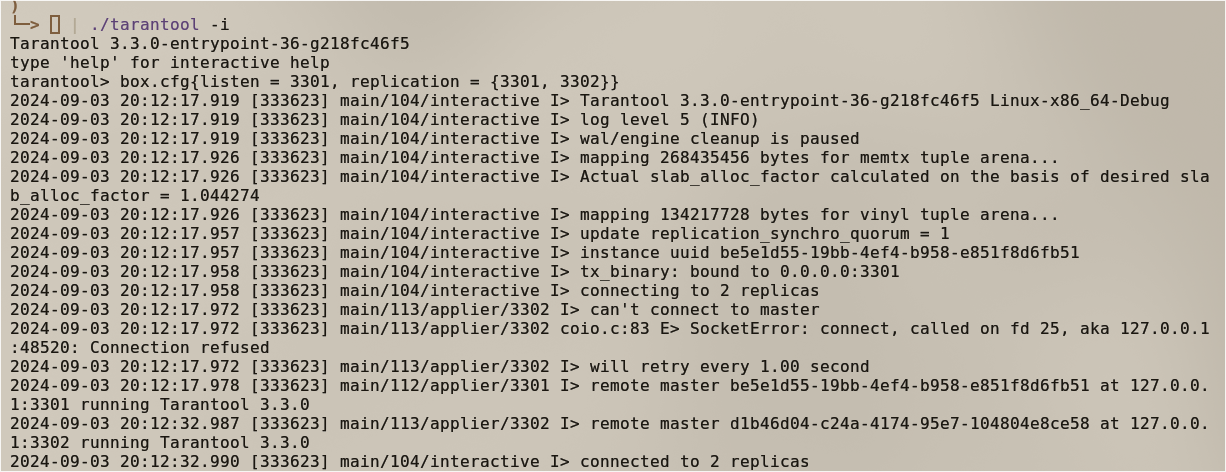
\includegraphics[scale=0.35]{inc/master.png}
  \caption{Конфигурация мастера}
  \label{fig:fig01}
\end{figure}

\textbf{Шаг 3. Конфигурация реплики}

Реплики настраиваются аналогичным образом, но с указанием опции \textit{read\_only}, устанавливающей режим только для чтения, чтобы запретить выполнение операций записи на реплике. Реплику можно сделать анонимной, указав параметр \textit{replication\_anon}.

\textbf{Шаг 4. Проверка состояния репликасета}

После настройки и запуска всех узлов необходимо убедиться, что репликасет работает корректно. Сделать это можно с помощью \textit{box.info.replication}, как показано на рисунке~\ref{fig:fig03}. Эта команда включает информацию о подключении к узлу, статусе синхронизации (\textit{vclock}) и задержке (\textit{lag}) \cite{TarantoolDoc}.

\begin{figure}
  \centering
  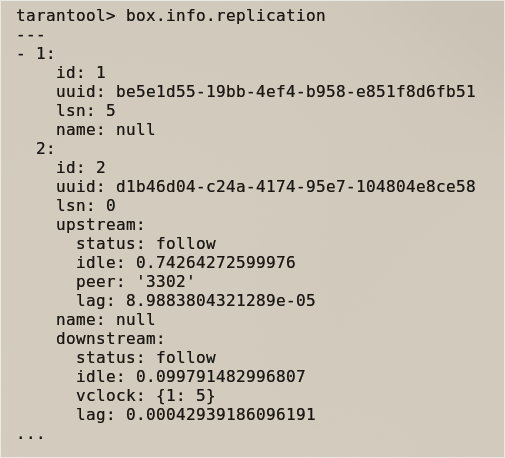
\includegraphics[scale=0.35]{inc/master-info.png}
  \caption{Состояние подключения узла}
  \label{fig:fig03}
\end{figure}


\subsection{Подключение узла к репликасету}

В данной части описывается протокол подключения реплики, так как это необходимо для понимания решений, предлагаемых к поставленным во введении задачам.

\begin{enumerate}
    \item В ходе конфигурации реплика генерирует UUID, являющийся уникальным идентификатором этого узла в репликасете. Для каждого URI в \textit{box.cfg.replication} создается сущность, называемая applier, задача которой состоит в применении данных, получаемых от мастера. Applier инициирует подключение к мастеру.
    \item Applier посылает сообщение IPROTO\_JOIN, при получении которого мастер создает relay, нужный для пересылки изменений БД на реплику. IPROTO\_JOIN представляет собой запрос на добавление узла к кластеру и необходим для получение начального состояния с мастера. Процесс отсылки начального состояния делится на две фазы.
    \item Initial JOIN. Мастер создает read-view (снимок) текущего состояние БД и посылает его реплике. По окончании initial JOIN мастер добавляет узел в репликасет путем вставки UUID реплики с соответсвующим ID в спейс \_cluster.
    \item Final JOIN. С момента создания read-view до окончания его пересылки может пройти много времени и состоянии БД наверняка изменится. Потому в фазе final JOIN мастер посылает все изменения, появившиеся со времени начала пересылки read-view.
    \item По окончании JOIN, реплика посылает запрос IPROTO\_SUBSCRIBE. Мастер отвечает своим текущим vclock-ом. С этого момента реплика переходит в стадию FOLLOW, она применяет все обновления WAL, исходящие от мастера.
\end{enumerate}

В Tarantool также есть возможность создания анонимных реплик, которые не являются участником репликасета, не могут становиться мастером, не учавствуют в кворуме синхронной репликации. Однако они получают и применяют поток репликационных данных. Вместо IPROTO\_JOIN они посылают IPROTO\_FETCH\_SNAPSHOT, который выполняет только первую фазу подключения: initial JOIN. Анонимные реплики не добавляются в спейс \_cluster. В любой момент анонимная реплика может стать обычной, послав запрос IPROTO\_REGISTER.

    \section{Файловый JOIN}

Одним из требований заказчика является возможность продолжения подключения реплики (JOIN) к репликасету с места остановки в случае сбоя. Эта функциональность будет обеспечиваться так называемым файловым JOIN, подробности которого описаны в данной части. Он работает только для анонимных реплик, что достаточно для CDC.

Такое требование вызвано большим временем выкачивания read-view во время стадии initial JOIN, в течение которого могут происходить многочисленные ошибки сети. Однако продолжить скачивание после переподключения нельзя, так как read-view нигде не сохраняется.

Вместо read-view было принято решение использовать файлы snapshot для отсылки изначального состояния. Это делается с помощью модификации протокола запроса IPROTO\_FETCH\_SNAPSHOT, который отныне выглядит следующим образом:

\begin{enumerate}
    \item Реплика посылает запрос IPROTO\_FETCH\_SNAPSHOT, указывая IPROTO\_CURSOR (описание см. ниже).
    \item Мастер отвечает на IPROTO\_FETCH\_SNAPSHOT vclock-ом снапшота, который он собирается посылать.
    \item После чего следует пересылка данных, каждая запись которых промаркирована с помощью LSN.
    \item В случае обрыва подключения, реплика посылает VCLOCK, полученный в пункте б, и LSN, до которого она успела получить данные.
\end{enumerate}

Так как vclock и данные с LSN уже посылались и до этого, именяется только IPROTO\_FETCH\_SNAPSHOT, приведенный в листинге 1.

\listing[
    caption={Изменения в запросе IPROTO\_FETCH\_SNAPSOT}
]{inc/fetch_snapshot_file_join.yaml}

Добавляется новое поле в тело запроса: IPROTO\_CURSOR, представляющее собой таблицу с полями VCLOCK и LSN. Она указывает, откуда необходимо продолжить скачивание файла. Она может иметь следующие значения:

\begin{itemize}
    \item \textit{\{nil, nil\}} - используется скачивания read-view для обратной совместимости
    \item \textit{\{\{0\}, 0\}} - курсор неизвестен, мастер берет последний сделанный snapshot и посылает его.
    \item \textit{\{VCLOCK, LSN\}} - курсор известен реплике и она хочет продолжить скачивание. Находим snapshot, идентифицируемый vlock-ом и начинаем пересылку с определенного LSN.
\end{itemize}

Мастер при получении IPROTO\_CURSOR проверяет, что снапшот с запрашиваемым vclock-ом еще существует и что в нем есть запрашиваемый LSN. В противном случае реплике возвращается ошибка, она должна снова передать \textit{\{\{0\}, 0\}} и начать скачивание уже другого снапшота заново.

    \section{Персистентный GC}

Следующим требованием заказчика было сохранение данных для анонимных реплик. Эта функциональность будет обеспечиваться персистентным GC, описание которого приводится в данной части.

Это требование вытекает из того факта, что репликация идет только из xlog файлов. Мастер постоянно отслеживает, кому и какие xlog файлы нужны в репликасете, и не удаляет их. Однако для анонимных реплик это не делается, так как они не входят в репликасет. Когда xlog файлы, которые еще не были среплицированы на анонимную реплику, удаляются, то реплика вынуждена делать процесс ребутстрапа, включающий в себя выкачивание состояния БД с нуля. Это приводит к существенному понижению доступности анонимной реплики.

Было принято решение полностью переделать систему GC, так как до этого состояние GC находилось в памяти и после перезапуска узел не знал, какие файлы нужно сохранять, а какие можно удалять. Это приводило к тому, что узел был вынужден ждать подключения всех реплик к текущему узлу.

\textbf{Локальный спейс \_gc\_consumers}

Теперь состояние GC сохраняется в новом локальном спейсе \_gc\_consumers, который имеет следующий формат, приведенный в таблице~\ref{tab:tab1}.

\begin{table}
    \centering
    \caption{Формат \_gc\_consumers}
    \begin{tabular}{|r|c|l|}\hline
        Поле & Имя & uuid \\ \hhline{~--}
             & Тип & string \\ \hline
        Поле & Имя & vclock \\ \hhline{~--}
             & Тип & map    \\ \hline
    \end{tabular}
    \label{tab:tab1}
\end{table}

UUID используется вместо id реплики, так как отныне xlog файлы могут также сохраняться для анонимных реплик, у которых id равно 0. Объединение всех анонимных реплик в одну строку не является оптимальным решением.

Для каждой из реплик создается GC consumer, который отслеживает, до какого vclock реплика уже получила данные. Их реализация (в памяти) остается без изменений, однако теперь они создаются\/удаляются с использованием on\_replace триггера спейса \_gc\_consumers. Во время запуска узла они будут созданы автоматически.

\textbf{Подключение обычных реплик}

Для обычных реплик появляется новый on\_replace триггер на спейс \_cluster, в который реплика вставляется после окончания фазы initial JOIN. Этот тригер вставляет кортеж в спейс \_gc\_consumers, что вызовет создание GC consumer для данной реплики. Удаление реплики из спейса \_cluster вызывает удаление записи из \_gc\_consumers. Прямое удаление реплики из \_gc\_consumers запрещено.

Таким образом, процесс подключение неанонимной реплики выглядит следующим образом:

\begin{enumerate}
    \item Реплика хочет быть присоединенной к репликасету и отправляет IPROTO\_JOIN.
    \item Мастер создает read-view, посылает его реплике. Реплика вставляется в спейс \_cluster, on\_replace триггер создает запись в \_gc\_consumers. Отныне файлы сохраняются для этой реплики.
    \item Реплика входит в фазу FOLLOW.
\end{enumerate}

\textbf{Подключение анонимных реплик}

Так как анонимная реплика нигде не сохраняется, как это делается для обычных реплик (\_cluster), нам необходимо добавить новый флаг в IPROTO\_FETCH\_SNAPSHOT: IPROTO\_IS\_PERSISTENT\_GC. По умолчанию флаг равен false, GC consumer-ы для анонимных реплик не создаются. Также этот флаг необходимо добавить в IPROTO\_SUBSCRIBE (инициация фазы FOLLOW).

Таким образом, процесс подключения анонимной реплики выглядит следующим образом:

\begin{enumerate}
    \item Реплика отправляет IPROTO\_FETCH\_SNAPSHOT с флагом IPROTO\_IS\_PERSISTENT\_GC. Реплика получает в ответ read-view или файл. Отныне xlog файлы хранятся для нее.
    \item Реплика отправляет IPROTO\_SUBSCRIBE с тем же флагом.
\end{enumerate}

Однако мы не можем позволить таким GC consumer-ам существовать вечно, как это сделано для обычных реплик. Иначе место на диске может быть быстро израсходовано. А потому добавляется новая опция конфигурирования: wal\_anon\_gc\_timeout. Она показывает, сколько секунд живет GC consumer, после момента, когда мы в последний раз общались с репликой.

    \section{Фильтрация репликационного потока}

Поcледним требованием заказчика была фильтрация репликационного потока. Это требование вытекает из необходимости снижения нагрузки на CDC реплики и заключается в частичной пересылки данных мастером.

Основные моменты:

\begin{itemize}
    \item Фильтрация репликации производится по именам спейсов. Фильтруется как процесс подключения реплик, так и процесс применения изменений. Клиент может подписаться на изменения спейсов, которые еще не были созданы.
    \item Запрошенные спейсы реплицируются вместе с их метаданным: \_space, \_index, \_truncate частично реплицируются, только данные, относящиеся к запрошенным спейсам, будут отправлены.
    \item При изменении имени или удаление спейса клиент получает информацию об этом последней записью. Последующие изменения (в случае переименования) не посылаются. Если будет создан спейс с именем, который запрошен клиентом, то клиент начинает получать данные из него.
\end{itemize}

Для обеспечения фильтрации в IPROTO\_FETCH\_SNAPSHOT и IPROTO\_SUBSCRIBE добавляется новая опция: IPROTO\_SPACE\_NAME\_FILTER, представляющая собой массив названий необходимых спейсов. Если опция не указана, полная репликация используется для обратной совместимости.

Управление подпиской на фильтрованный репликационный поток:

\begin{itemize}
    \item Добавление нового еще не существующего спейса к фильтру. Клиент может инициировать IPROTO\_SUBSCRIBE в любой момент, чтобы добавить новый спейс.
    \item Удаление спейса из фильтра. Делается таким же образом.
    \item Добавление уже существующего спейса в фильтр. Недопустимое изменение фильтра. На момент изменения фильтра клиент уже имеет какой-то vclock и мы продолжим посылать данные с этого vclock-a. Однако метаданные спейса будут скорее всего пропущены, так как спейс уже был создан до изменения фильтра.
\end{itemize}


    \conclusion

Таким образом, в ходе прохождения практики был разработан новый протокол подключения анонимных реплик, удовлетворяющий требованиям команды CDC. Он выглядит следующим образом:

\begin{enumerate}
    \item Анонимая реплика отправляет IPROTO\_FETCH\_SNAPSHOT, сообщая мастеру, что она хочет реплицироваться с него. В этот запрос может быть включены следующие опции:
    \begin{enumerate}
        \item IPROTO\_CURSOR - реплика хочет использовать файловый JOIN для возможности продолжения подключения в случае разрыва подключения.
        \item IPROTO\_IS\_PERSISTENT\_GC - необходимо создать анонимного GC consumer и сохранять xlog файлы для данной реплики.
        \item IPROTO\_SPACE\_NAME\_FILTER - поток репликации должен быть фильтрованным. Требуются только частичные данные.
    \end{enumerate}
    \item В ответ мастер посылает vclock read-view или файла снапшота (в зависимости от IPROTO\_CURSOR). Мастер создает анонимный GC consumer, если опция IPROTO\_IS\_PERSISTENT\_GC равен true.
    \item Мастер начинает пересылку данных. Если IPROTO\_SPACE\_NAME\_FILTER указан, то данные фильтруются на стороне сервера и посылаются частично.
    \item Реплика посылает IPROTO\_SUBSCRIBE, указывая необходимость GC consumer и фильтрации потока.
\end{enumerate}

В любой момент времени процесс подключения может быть разорван и продолжен с того же момента. Ошибки удаления файлов xlog больше не возникают, так как теперь есть возможность их сохранения для анонимных реплик. Нагрузка на CDC реплики была снижена, так как теперь им больше не приходится самостоятельно обрабатывать фильтрацию репликации.


    \printbibliography
\end{document}
